\documentclass[conference,9pt]{IEEEtran}
\usepackage{color}
\usepackage{cite}
\usepackage{epsfig}
\usepackage{amssymb}
\usepackage{amsmath}
\usepackage{graphicx}
\graphicspath{ {../} }

\begin{document}
%\tableofcontents
%\textheight=22.6cm
%
% paper title
\title{Practical 1A}

% author names and affiliations
\author{
\IEEEauthorblockN{Albert Acebron}
\IEEEauthorblockA{NIU: 1458626}
}


% make the title area
\maketitle
\begin{abstract}
This practical will be based around applying a matched filter to a signal distorted by AWGN\end{abstract}



%----------------------------------------------------------------
% SECTION #1 
\section{Introduction}
The main objective of this practical will be the application of a matched filter, which will involve some analysis of the pattern signal we are trying to find, along with which filters would work best on it, and the implementation of an algorithm that enables us to apply said filter on long or infinite sequences in a computationally inexpensive way.

\section{Questions}
\subsection{Question 1}
\begin{verbatim}
senyal_conformat = pam_sqrrc(25, 20, 0.35, 1)
plot(1:length(senyal_conformat),
    senyal_conformat)
\end{verbatim}
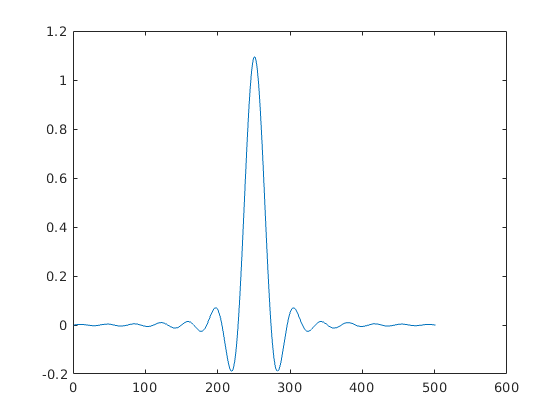
\includegraphics[scale=0.6]{pulso1}

\subsection{Question 2}
The definition of a matched filter h[x] is a filter that, when convoluted with the input signal, generates an output signal that has a maximum SNR (under the assumption that AWGN is causing interferences).

By taking the definition of convolution and SNR, we can formulate SNR as a function of the filter being applied to a function and then proceed to optimize it. Doing so will yield that the filter that achieves this optimuum is a conjugated and time-reversed version\cite{proof} of the signal we are trying to match/find, which in this case is the SQRRC pulse.

In conclusion, the filter we should use is a conjugated and time-reversed SQRRC pulse.

\subsection{Question 3}
The SQRRC pulse doesn't have any imaginary components, so there's no need to conjugate it. For that reason we will simply revert it on the time scale, which should wield the same figure, since the pulse is symmetric against x=0.

Now we'll proceed to calculate the total energy:
\begin{verbatim}
energy = sum(senyal_conformat.^2)
\end{verbatim}
This resolves to 24.99, which is clearly not 1. If we would like it to be we could just introduce a linear multiplicative constant $\beta$:
$$newSignal = signal\cdot \beta$$
$$energy = \sum (signal\cdot beta)^2$$
And constraint $energy$ to be 1:
$$1 = \sum (signal\cdot beta)^2$$
$$1 = \dfrac{\sum signal^2}{\dfrac{1}{beta^2}}$$
$$beta^2 = \dfrac{1}{\sum signal^2}$$
$$beta = \sqrt{\dfrac{1}{\sum signal^2}}$$

Which calculated would be:
\begin{verbatim}
beta = sqrt(1/sum(senyal_conformat.^2))
\end{verbatim}
That evaluates to 0.2.

In conclusion, the amplitude of the filter would need to be multiplied by 0.2 to get the total energy of it to be 1.

\subsection{Question 4}
\begin{verbatim}
function FilteredSignal = overlap_add(RxSignal, h)

M=length(h);
Lr=length(RxSignal);
L=(M-1)*2; % Taken from the recomendation on the practical
N=L+M-1;
Hx=fft(h, N);
FilteredSignal=zeros(Lr+M-1, 1);

for x = 0:floor(Lr/L)
    len=L;
    initialPos=x*L+1
    if (initialPos+len)>(Lr-1)
        len=Lr-initialPos
        N=len+M-1;
        Hx=fft(h, N);
    end
    r=RxSignal(initialPos:initialPos+len-1);
    Rm=fft(r, N);
    Ym=Rm.*Hx;
    ym=ifft(Ym, N);
    endFiltered=initialPos+length(ym)-1;
    FilteredSignal(initialPos:endFiltered)=FilteredSignal(initialPos:endFiltered)+ym;
end
\end{verbatim}

\subsection{Question 5}
The plot is generated with:
\begin{verbatim}
t1=triang(10)
t2=triang(30)
hold on
plot(conv(t2,t1))
plot(add(t2,t1))
\end{verbatim}

The result is not really clear but the two superimposed figures are right on top of each other:

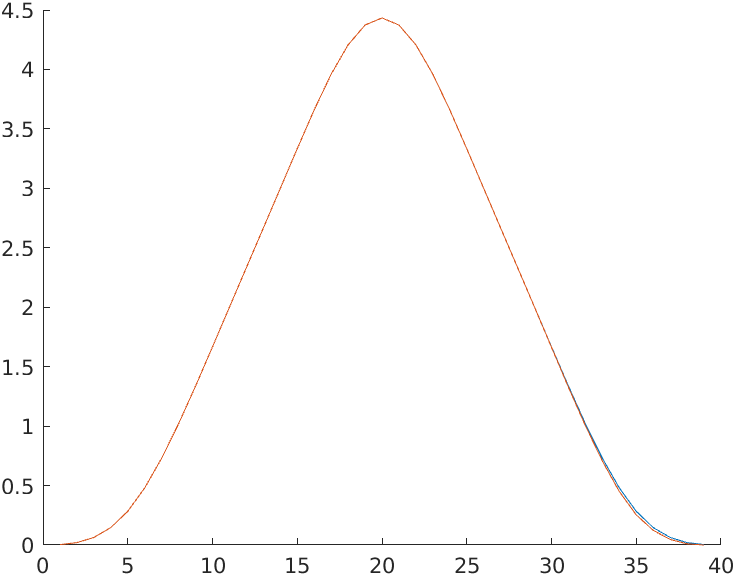
\includegraphics[scale=0.6]{comp}

\section{Conclusion}
We managed to both construct the matched filter that should be used to remove noise and implement an algorithm to apply it to our input signal, thus accomplishing the task of finishing the first section of the signal processing pipeline that is being evaluated on this practical.

\begin{thebibliography}{1}
\bibitem{proof}
https://en.wikipedia.org/wiki/Matched\_filter\#Derivation\_via\_matrix\_algebra
\end{thebibliography}

% that's all folks
\end{document}


